% ===========================================================================
%
%		FEDERICO II THESIS TEMPLATE - ENGLISH
%  					* an example of Chapter 1: information about the discussion of the thesis
%	 
% 		AUTHOR:  		Antonio Esposito (antonio.esposito103@studenti.unina.it)
%		LAST UPDATED:	2017/06/20
%
% ===========================================================================

\chapter{Modello di Dominio}

%%%%% ===============================================================================
\section{Classi, oggetti e relazioni di analisi}
Si riportano di seguito i Class Diagram di analisi dei casi d'uso.
\includepdf[pages={-}]{Class Diagram/Analisi/CD-Analisi-tutti.pdf}
%%%%% ===============================================================================
\section{Diagrammi di sequenza di analisi}
Si riportano di seguito i diagrammi di sequenza di analisi dei casi d'uso.
%\includepdf[pages={1-6}]{SequenceAnalisi/diagrammi.pdf}

\pagebreak
%%%%% ===============================================================================
\section{Diagrammi di stato di analisi}
Sono riportati di seguito i diagrammi di stato di alcuni casi d'uso.
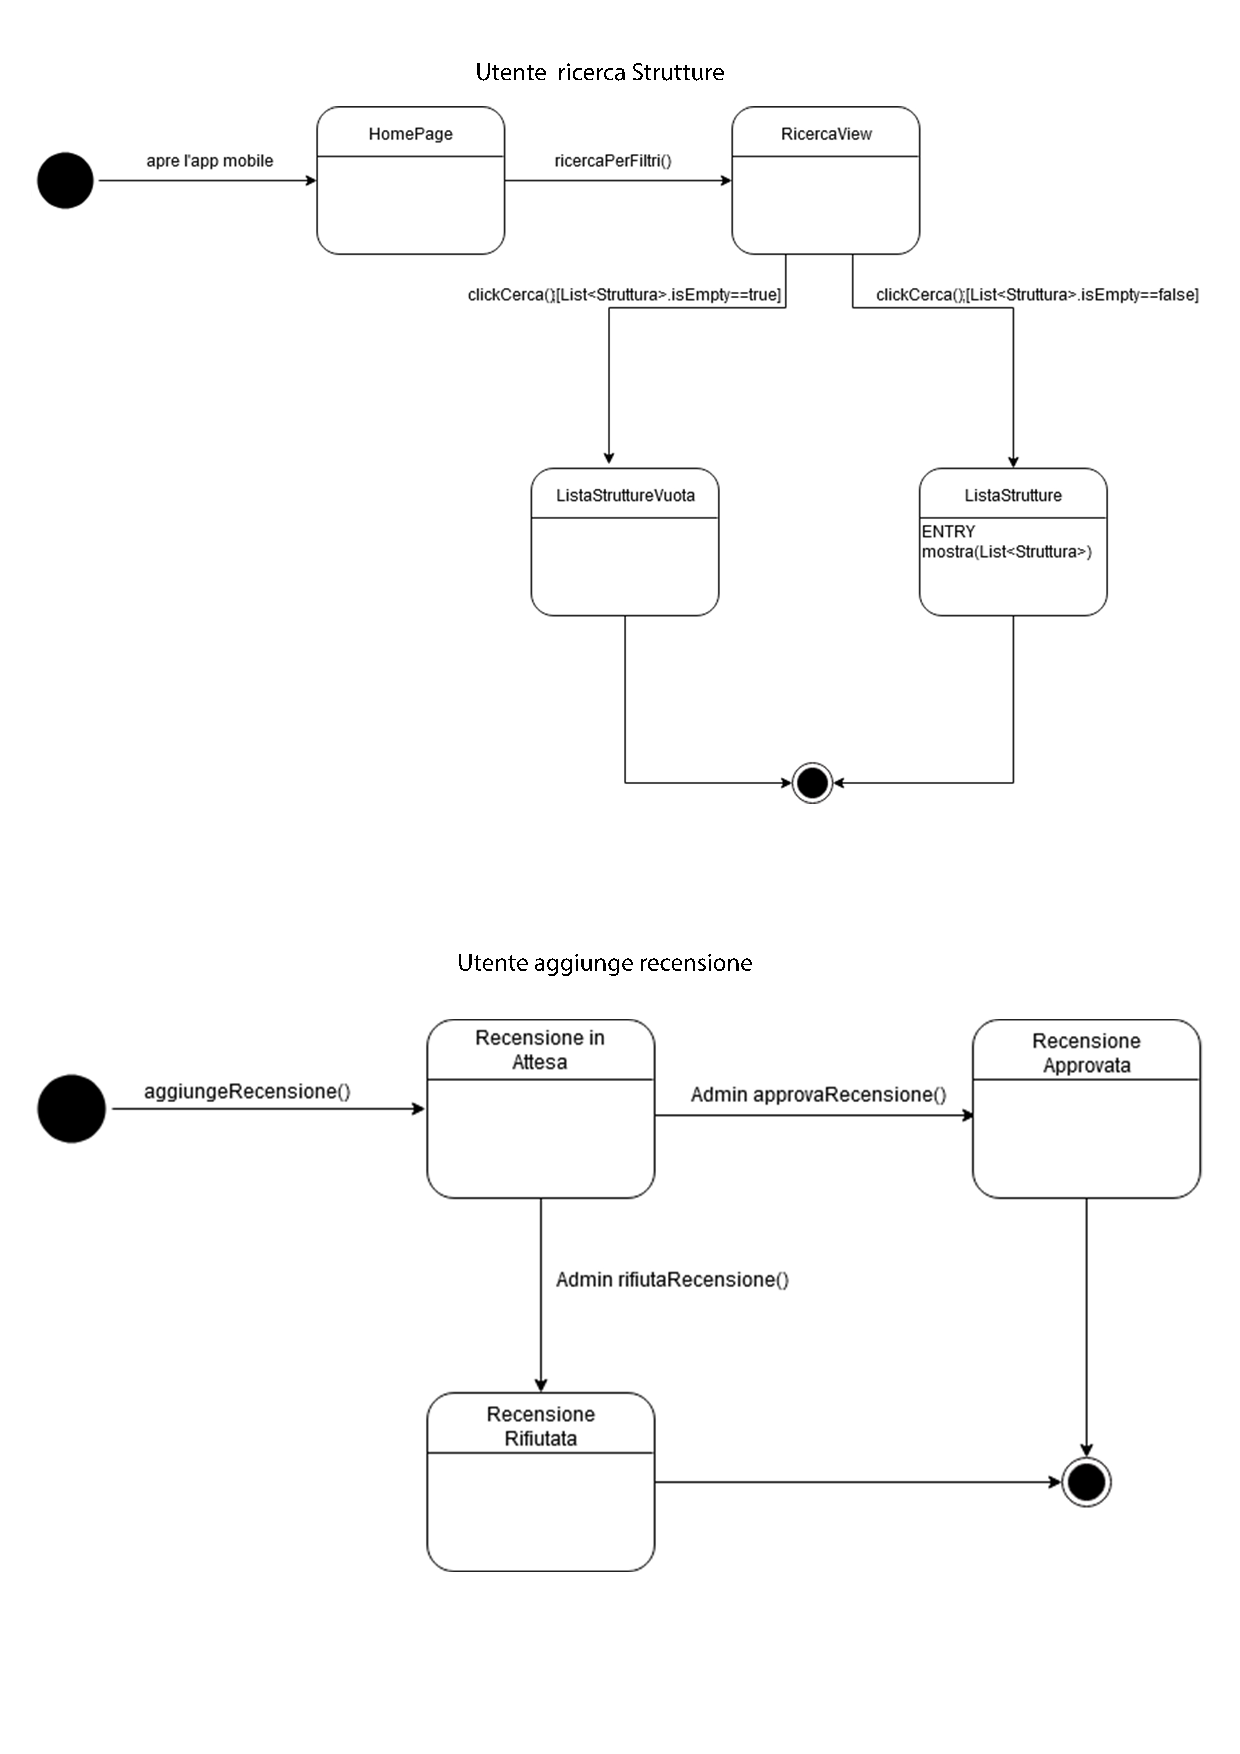
\includepdf[pages={-}]{State Chart/Analisi/state chart.pdf}
\pagebreak
%%%%% ===============================================================================
\section{Diagrammi di attività di analisi}
Sono riportati di seguito i diagrammi di attività di alcuni casi d'uso.
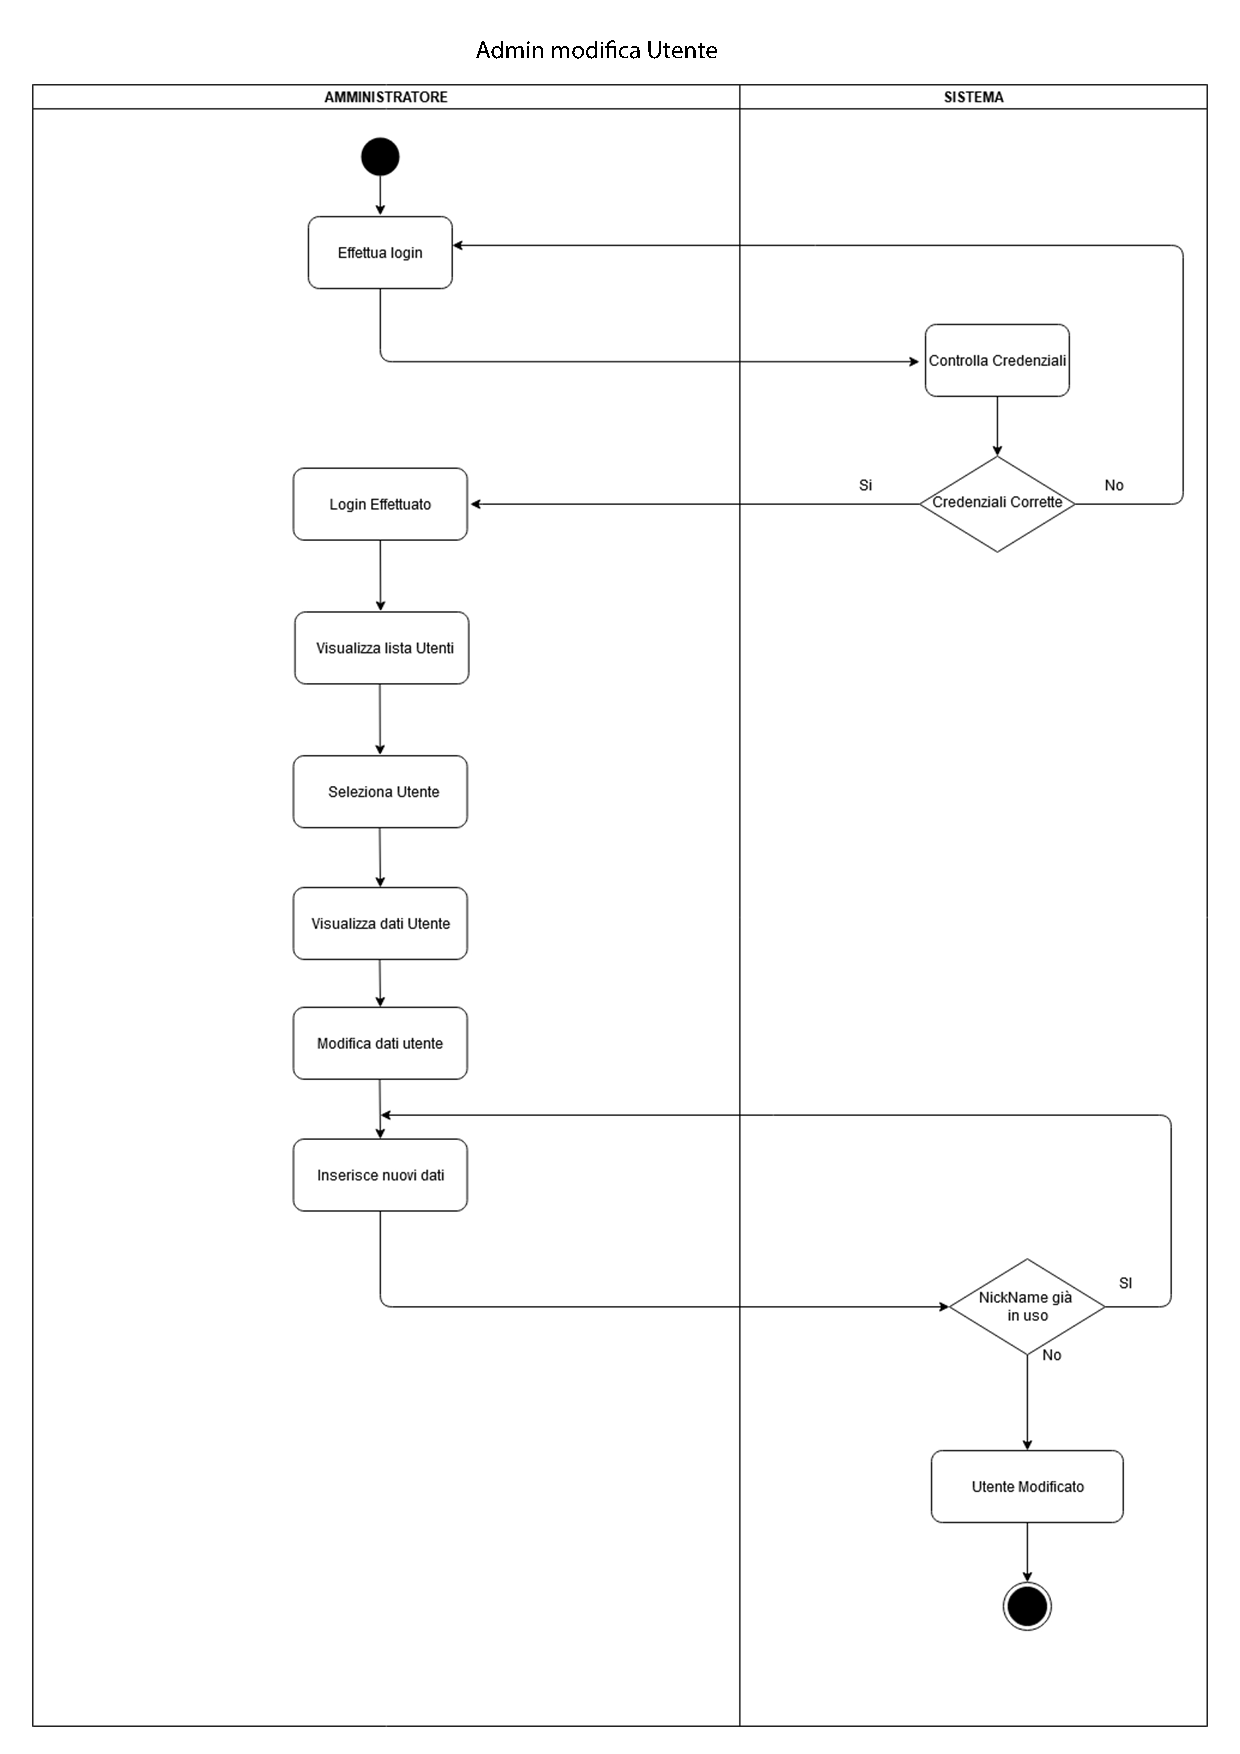
\includepdf[pages={-}]{Activity Diagram/Activity Diagrams.pdf}

%%%%% ===============================================================================
